\documentclass[../../main]{subfiles}
\begin{document}

\begin{figure}[h!]
\[
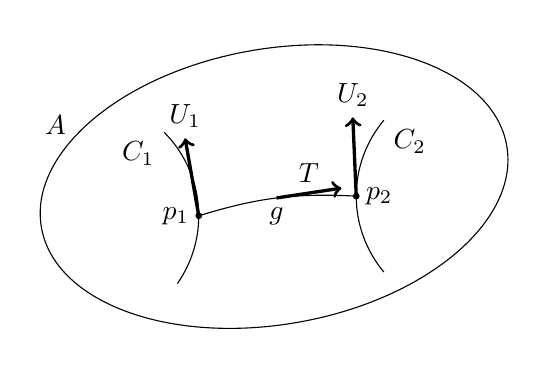
\begin{tikzpicture}
    \coordinate (P1) at (-1,-0.125);
    \coordinate (P2) at (1,0.125);
    
    %geodesic
    \draw (P1)
        to[bend left=10] 
        coordinate[midway](G) 
        node[midway, anchor=north] {$g$}
        (P2);
    \draw[very thick, ->] 
        (G) 
        to 
        node[midway, anchor=south] {$T$}
        ++(0.825,0.125);
    
    %surfaces at p_1, p_2
    \draw (P1) arc (0:45:1.5cm) node[anchor=north east] {$C_1$};
    \draw (P1) arc (0:-35:1.5cm);
    
    \draw (P2) arc (180:140:1.5cm) node[anchor=north west] {$C_2$};
    \draw (P2) arc (180:220:1.5cm);
    
    \draw[very thick, ->] (P1) to ++(100:1) node[anchor=south] {$U_1$};
    \draw[very thick, ->] (P2) to ++(92.5:1) node[anchor=south] {$U_2$};
    
    \foreach \i/\j in {1/east,2/west}
    {
        \filldraw (P\i) circle (1pt) node[anchor=\j] {$p_\i$};
    }
    
    \draw[rotate=10] (0,0.25) ellipse (3cm and 1.75cm);
    \draw (160:3) node {$A$};
\end{tikzpicture}
\]
\caption{Cross Manifolds}
\label{fig:ch10fig4}
\end{figure}

\end{document}